%Author: xbielg00, xtobol06, xgabry01, xmikys03
%Author: xbielg00, xtobol06, xgabry01, xmikys03

%class
\documentclass[a4paper, 12pt]{article}

%encoding
\usepackage[T1]{fontenc}           %font encoding
\usepackage[utf8]{inputenc}         %script encoding

%packages
\usepackage[czech]{babel}           %language
\usepackage[a4paper, text={17cm,24cm}, left=2cm, top=3 cm]{geometry}		%layout
\usepackage{times}					%font
\usepackage[ruled, czech, linesnumbered, longend, noline]{algorithm2e}		%algorithms
\usepackage[unicode,hidelinks]{hyperref}	%links
\usepackage{amsmath}
\usepackage{tabularx}
\usepackage{multicol}
\usepackage{multirow}
\usepackage{graphicx}
\usepackage{float}
\usepackage{csquotes}
\usepackage[htt]{hyphenat}
\usepackage[htt]{hyphenat}

\begin{document}

    \begin{titlepage}
		\centering

        
\includegraphics{src/fitlogo.pdf}

        \vspace{\stretch{0.382}}

        {\Huge Dokumentace k projektu z IFJ a IAL\\[0.4em]
            \LARGE Tým xbielg00, varianta TRP}

        \vspace{\stretch{0.618}}

        \begin{table}[H]
            \hfill
            \begin{tabularx}{0.5\textwidth}{Xr}
                \textbf{Gabriel Biel} & \textbf{xbielg00 }\ \ \ 30\%\\
                Adam Gabrys & xgabry01  \ \ \ 15\% \\
                Jakub Mikyšek & xmikys03  \ \ \ 25\% \\
                David Tobolík & xtobol06  \ \ \ 30\% \\
                \textbf{Gabriel Biel} & \textbf{xbielg00 }\ \ \ 30\%\\
                Adam Gabrys & xgabry01  \ \ \ 15\% \\
                Jakub Mikyšek & xmikys03  \ \ \ 25\% \\
                David Tobolík & xtobol06  \ \ \ 30\% \\
            \end{tabularx}
        \end{table}
	\end{titlepage}

    \tableofcontents
    \newpage

    \section{Úvod}
    Cílem našeho projektu bylo vytvoření překladače jazyka IFJ22, který je poupravenou podmnožinou jazyka PHP. Námi vytvořený překladač jsme implementovali v jazyce C a  má za úkol daný zdrojový kód načíst a zpracovat několika způsoby, kdy je zapotřebí využití lexikální, syntaktické, precedenční a sémantické analýzy s následným přeložením do mezikódu IFJcode22, který již zpracovává předem poskytnutý interpret, který tento mezikód provádí.

    \section{Popis fungování a struktura překladače}
    Překladač se skládá z několika propojených spolu fungujících částí, kdy každá z nich zastává důležitou roli. Jde tedy o lexikální, syntaktickou, sémantickou a precedenční analýzu, po jejímž průchodu zastává důležitou část také generování mezikódu IFJcode22. Bylo nutné si překladač rozdělit do těchto částí, aby bylo jasné, které funkce překladače daná část zastává a lépe se nám dělila práce v týmu.

     \section{Lexikální analýza}
    Lexikální analýza (dále LA) načítá lexémy ze standardního vstupu pomocí funkce \texttt{getToken()}, ty následně přetváří na tokeny, které postupně naplňují list \texttt{TokenList}. List se po zpracování vstupu předává syntaktické analýze. LA se volá funkcí \texttt{lexAnalyser()} a je implementovaná v souborech \texttt{lex\_analyzer.c} a \texttt{lex\_analyzer.h}. Zpracování lexémů se řídí předem vytvořeným deterministickým konečným automatem (viz \ref{Konecny automat}). Konečný automat je reprezentován v LA  switchem, u kterého každý case zastupuje jeden jeho stav. Pokud automat natrefí na nesouvisející vstupní hranu a nachází se v konečném stavu, spouští se funkce \texttt{tokenCtor()} pro vytvoření tokenu a poté \texttt{appendToken()} pro vložení do seznamu tokenů. Pokud se ale automat nenachází v konečném stavu, LA hlásí lexikální chybu a překlad se ruší. O tokenu se uchovává informace o jeho typu, číslo řádku\,--\,na kterém se token nalézal a relevantní data (název proměnné, funkce, hodnota atd.).
    \section{Syntaktická analýza}

    \subsection{Rekurzivní sestup} \label{sestup}
        Rekurzivní sestup se volá funkcí \texttt{synAnalyser()} a je implementovaný v souborech \texttt{syn\_analyzer.c} a \texttt{syn\_analyzer.h}. Řídí se podle navržené gramatiky (viz \ref{LL gramatika}), kde každé pravidlo představuje vlastní funkci. Funkce postupně prochází tokeny získané od lexikální analýzy, kontroluje jestli je vše gramaticky správně, naplňuje tabulku symbolů a tvoří abstraktní syntaktický strom (dále ASS). Při nalezení výrazu volá funkci \texttt{parseExpression}, která spouští precedenční analýzu. Při nalezení chyby se nastaví příslušný \texttt{errorCode} a chyba se v rekurzi propaguje dál, aby program ukončil kontrolu. Funkce vrací vytvořený ASS, naplněnou tabulku symbolů a informaci o tom, jestli rekurze proběhla syntakticky a sémanticky správně či nikoliv.

    \subsection{Precedenční analýza}
    Soubory \texttt{preced\_analyzer.c}, \texttt{preced\_analyzer.h}, \texttt{preced\_analyzer-data.h}

    Na zpracování výrazů jsme použili metodu shora-dolů - precedenční analýzu (dále jen PA). PA kontroluje sémantiku volání funkcí a zda byly použité proměnné definovány. Ke kontrole využívá tabulku symbolů. Dále se od sémantických kontrol zabývá PA také správnou syntaxí zadaného výrazu pomocí zásobníku PA a precedenční tabulky (viz \ref{tabulka precedence}). Výrazy se redukují pomocí pravidel, které máme definovány v souboru \texttt{preced\_analyzer.c}. Výstupem PA je post-fixově zpracovaný výraz na zásobníku ASS.

    \section{Tabulka symbolů}
    Soubory \texttt{symtable.c}, \texttt{symtable.h}

    Pro implementaci tabulky symbolů jsme si ze zadání vybrali variantu TRP, tedy tabulku s rozptýlenými položkami, kdy jsme při jejím tvoření využili získané znalosti, jak z přednášek, tak z projektu do předmětu IAL. Pro práci s položkami jsme využívali hlavně funkci \texttt{ht\_insert()}, kdy při vkládání položky do tabulky jsme rozdělovali, zda vkládáme funkci, či proměnnou. Obecně jsme si ukládali ID - unikátní řetězec, který slouží jako klíč. Dále počet referencí na položku a odkaz na další položku v tabulce. Pokud byla daná položka funkce, ukládali jsme si navíc její návratový typ a informace o parametrech jí přiřazené, to pomocí funkce \texttt{ht\_paramAppend()}.
    Pro správnou funkcionalitu tabulky jsme museli samozřejmě implementovat i další funkce, jako například odstranění položky z tabulky/odstranění všech položek (funkce \texttt{ht\_delete()}, \texttt{ht\_delete\_all()}) a ostatní, které jsou detailně popsány v souboru
    \texttt{symtable.h} a implementovány v souboru \texttt{symtable.c}.

    \section{Abstraktní syntaktický strom}
    Soubory \texttt{ast.c}, \texttt{ast.h}

    Abstraktní syntaktický strom (dále ASS) je implementovaný jako zásobník (viz \ref{zasobniky}), který obsahuje strukturu pro ASS. Ta je tvořena typem a volitelnými daty.
    \begin{itemize}
        \item Aritmetické, řetězcový a relační operátory\,--\,každý má svůj typ, nemají data, na zásobníku předcházejí 2 operandy.
        \item Přiřazení\,--\,nemá data, na zásobníku následuje proměnná, do které se přiřazuje a po ní výraz nebo volání funkce, které se má přiřadit.
        \item Proměnná\,--\,v datech obsahuje ukazatel do tabulky symbolů.
        \item Konstanty\,--\,každý typ konstanty má svůj typ v ASS (int, string, float, null) a obsahuje, kromě typu null, hodnotu této konstanty.
        \item Deklarace funkce\,--\,v datech je uložený ukazatel do tabulky symbolů na tuto funkci.
        \item Volání funkce\,--\,v datech obsahuje ukazatel na strukturu volání funkce, v ní je uložen ukazatel do tabulky symbolů a seznam parametrů. Parametry mají rovněž typ (proměnná nebo konstanta\,--\,int, string, float, null) a svoje data (ukazatel do tabulky symbolů nebo hodnota konstanty).
        \item Volání return\,--\,typ bez návratové hodnoty nebo s návratovou hodnotou, v tom případě na zásobníku následuje výraz, který se má vrátit.
        \item Podmínky\,--\,if, else, while\,--\,nemají data, na zásobníku následuje výraz, který je v podmínce.
        \item Konec výrazu\,--\,značí konec výrazu nebo volání funkce, slouží k rozpoznání konce postfixového zápisu.
        \item Konec složeného výrazu\,--\,značí konec složeného příkazu ve složených závorkách (if, else, deklarace funkce).
    \end{itemize}
    Řídící struktury jsou uloženy prefixově, výrazy postfixově, toho se s výhodou využívá v generování kódu (viz \ref{generovani}).
    \section{Zásobníky} \label{zasobniky}
    Soubory \texttt{stack.c}, \texttt{stack.h}

    Zásobníky byly potřeba na více místech (ASS, precedenční analýza, generování kódu, \ldots). Implementace zásobníků je tedy obecná pomocí makra, které je možné použít pro libovolný ukazatel. Pro operaci pop je potřeba v makru specifikovat destruktor, který správně uvolní prvek, což je vhodné především pro komplexnější struktury. Při tvorbě ASS je potřeba, aby byl začátek programu na vrcholu zásobníku, proto je zásobník rozšířen o funkci, která umožňuje vložení prvku na konec zásobníku, aby se ASS do zásobníku mohl vkládat sekvenčně.

    \section{Sémantické kontroly}
    Všechny sémantické kontroly probíhají s pomocí tabulky symbolů. Před spuštěním syntaktické analýzy, proběhne tzv. \uv{první průchod} za pomocí funkce \texttt{fncDeclarationTable}, která kontroluje jen definice funkcí a nahrává je společně s jejich parametry a návratovým typem do tabulky symbolů. V návaznosti na tento první průchod se v precedenční analýze při volání funkcí provádí kontrola typu a počtu parametrů nebo zda byla funkce definována. Sémantické kontroly pro proměnné a jejich (ne)definování se provádějí v syntaktické a precedenční analýze.

    \section{Generování kódu} \label{generovani}
    Soubory \texttt{code\_gen.c}, \texttt{code\_gen.h}, \texttt{code\_gen\_static.c}, \texttt{code\_gen\_static.h}

    Generování kódu zajišťuje funkce \texttt{codeGenerator}, která slouží jako kontroler celého generování. Předává si řízení s funkcemi, které slouží pro generování konkrétních částí, stará se o správu kontextu programu, uvolnění dat apod.

    Byly domluveny konvence předávání hodnot volání funkcí, pomocných funkcí (viz \ref{pomocne}) a vyhodnocených výrazů. Parametry vestavěných funkcí a funkcí definovaných uživatelem (kromě funkce write, která se generuje přímo) se předávají v předdefinovaných proměnných ve vytvořeném lokálním rámci. Lokální rámec připravuje a uklízí vždy volající. Pomocné funkce očekávávají parametry vždy na zásobníku, toto řešení jsme zvolili pro omezení vytváření rámců, s ohledem na malý počet parametrů těchto funkcí, které berou 1 nebo 2 parametry. Návratová hodnota se u všech funkcí a u výrazů předává na zásobníku.

    \subsection{Kontext programu}
    Funkce \texttt{codeGenerator} vytváří a aktualizuje kontext programu a předává ho některým funkcím. Kontext obsahuje čítače návěští, zásobník zanoření a ukazatel na aktuálně deklarovanou funkci. Zásobník zanoření obsahuje prvky, které identifikují typ a pořadí složených příkazů.

    \subsection{Statické funkce a definice proměnných}
    Před spuštěním veškerého generování kódu jsou vygenerovány statické části programu a definice proměnných. Statická část obsahuje definici globálních pomocných proměnných, které slouží místo registrů a definici vestavěných a pomocných funkcí. Tato část je přeskočena instrukcí \texttt{JUMP} až na začátek programu. Na začátku se vytvoří nový lokální rámec a nadefinují se všechny proměnné, které jsou použity v hlavním těle programu (i v podmínkách a cyklech, tudíž všude kromě deklarace funkcí).

    \subsection{Generování konkrétních částí programu}

    \subsubsection{Podmínky\,--\,\texttt{if else, while}}
    Podmínka \texttt{if} se na začátku vyhodnotí a v případě nepravdivosti výrazu v podmínce se skočí na návěští \texttt{else} doplněné pořadovým číslem z kontextu. Před návěští \texttt{else} se vygeneruje skok za složený příkaz. U cyklu \texttt{while} se vygeneruje návěští začátku cyklu (opět doplněné o pořadové číslo z kontextu), při neplatnosti podmínky skočí až za konec cyklu. Návěští konce složených příkazů \texttt{else} a \texttt{while} jsou generovány na konci složeného příkazu (viz \ref{konec slozeneho}).

    \subsubsection{Přiřazení}
    Nejdříve se vyhodnotí výraz, který se má přiřadit a potom se přiřadí výsledek ze zásobníku pomocí instrukce \texttt{POPS}.

    \subsubsection{Volání funkce}
    Před voláním funkce se vytvoří dočasný rámec, ve kterém se nadefinují a inicializují argumenty funkce. Před každým přiřazením proměnné do parametru se zkontroluje její inicializace. Zavolá se funkce, případně se přiřadí hodnota ze zásobníku a uklidí se rámec.

    \subsubsection{Deklarace funkce}
    Vygeneruje se příslušné návěští a definice lokálních proměnných použitých ve funkci, kromě jejich parametrů (ty jsou definovány při volání funkce). Celá deklarace se přeskočí instrukcí \texttt{JUMP}, aby její obsah nezasahoval do hlavní části programu.

    \subsubsection{Volání return}
    Podle kontextu se vygeneruje \texttt{EXIT} nebo návrat z funkce. Před navrácením hodnoty se zkontroluje její typ, poté se vloží na zásobník a vygeneruje se \texttt{RETURN}.

    \subsubsection{Výrazy}
    Výrazy využívají postfixového zápisu v ASS. Jednotlivé operandy se vkládají na zásobník a redukují operacemi na mezivýsledky případných dalších operací. Před každým použitím proměnné, se kontroluje její inicializace.

    \subsubsection{Konec složeného příkazu} \label{konec slozeneho}
    Když je na vrcholu zásobníku ASS konec složeného výrazu, vyhodnotí se následující akce podle typu složeného výrazu v kontextu.
    \begin{itemize}
        \item \texttt{if}\,--\,vygeneruje skok na konec složeného příkazu \texttt{else}.
        \item \texttt{else}\,--\,generuje návěští značící konec příkazu \texttt{else}.
        \item \texttt{while}\,--\,generuje skok na začátek cyklu a návěští konce cyklu.
        \item deklarace funkce\,--\,vygeneruje kontrola návratu z funkce, v případě \texttt{void} funkce se vygeneruje navrácení z funkce. Aktualizuje se kontext programu.
    \end{itemize}

    \subsection{Pomocné funkce pro vygenerovaný kód} \label{pomocne}
    Ve statické části se generují pomocné funkce, které se potom volají na příslušných místech v programu. Jedná se o implicitní typové konverze, vyhodnocování podmínek, kontrola typů apod.

    \section{Týmová spolupráce}
    \label{teamwork}
    \subsection{Komunikace v týmu}
        Vzájemná domluva a komunikace probíhala online i offline. A to prostřednictvím Discord serveru\,--\,pro převážně obecnější problematiky, pro ty složitější a již více konkrétní nám sloužila funkce GitHub Issues, kde jsme mohli jednoduše diskutovat o již konkrétní části kódu. K tomu jsme se každý čtvrtek setkávali na schůzích uskutečněných v budově školy, kde jsme řešili ty nejzásadnější problémy a rozhodnutí z hlediska směřování.
    \subsection{Verzovací systém}
        Při výběru verzovacího systému pro nás bylo jasnou volbou zvolit populární a osvědčený Git s nahráváním na server GitHub, kde probíhala i již zmíněná vzájemná komunikace.
    \subsection{Testování}
        Pro ověření správnosti jsme používali framework GoogleTest v jazyce C++, který nám sloužil k unit testování. Co se týče integračního testování, zde jsme zvolili cestu manuálních testů.
    \subsection{Rozdělení práce a bodů}
        \begin{itemize}
            \item Gabriel Biel (xbielg00)
                \begin{itemize}
                    \item architektura překladače, lexikální analýza, precedenční tabulka, precedenční analýza, testy pro precedenční analýzu, rozhraní pro tabulku symbolů, funkce v generátoru kódu
                    \item \textbf{30\%}
                \end{itemize}
            \item Adam Gabrys (xgabry01)
                \begin{itemize}
                    \item Konečný automat, sémantické kontroly pro deklarace funkcí, generování built-in funkcí, dokumentace
                    \item \textbf{15\%}
                    \item Konečný automat, sémantické kontroly pro deklarace funkcí, generování built-in funkcí, dokumentace
                    \item \textbf{15\%}
                \end{itemize}
            \item Jakub Mikyšek (xmikys03)
                \begin{itemize}
                    \item gramatika, LL tabulka, rekurzivní syntaktická analýza, sémantické kontroly pro proměnné, integrační testování pro parser, dokumentace
                    \item \textbf{25\%}
                    \item gramatika, LL tabulka, rekurzivní syntaktická analýza, sémantické kontroly pro proměnné, integrační testování pro parser, dokumentace
                    \item \textbf{25\%}
                \end{itemize}
            \item David Tobolík (xtobol06)
                \begin{itemize}
                    \item sémantické kontroly pro volání funkce, generování kódu, datové struktury pro ASS, zásobníky, pomocná makra a funkce, struktura projektu, cmake a struktura testů, testy (lexikální analýza, ASS, zásobníky), code review, makefile, dokumentace
                    \item \textbf{30\%}
                    \item sémantické kontroly pro volání funkce, generování kódu, datové struktury pro ASS, zásobníky, pomocná makra a funkce, struktura projektu, cmake a struktura testů, testy (lexikální analýza, ASS, zásobníky), code review, makefile, dokumentace
                    \item \textbf{30\%}
                \end{itemize}
        \end{itemize}
    \subsection{Důvod nerovnoměrného rozdělení bodů}
    Pro nerovnoměrné rozdělení bodů jsme se rozhodli jelikož někteří členové týmu odvedli proporčně značně větší část práce, a proto nám to takto přišlo fér a všichni členové týmu se na tomto rozdělení shodli.

    \section{Závěr}
    Projekt nás svým objemem ze začátku opravdu překvapil a chvíli nám trvalo, než jsme se zorientovali v zadání. Naštěstí nám opravdu pomohlo scházet se každý týden a prodiskutovat jednotlivé problémy, či náš pokrok v práci. Velkou část sehrálo také to, že jsme se všichni znali a komunikovali vcelku bez prodlev a problémů a to jak na GitHubu, tak na Discord serveru, který jsme si pro projekt vytvořili(viz \ref{teamwork}). Práce nám s odstupem času šla stále lépe, jelikož jsme rozuměli dané problematice i specifikacím zadání stále více. Projekt nám přinesl nejen znalosti do předmětů IFJ a IAL, ale velmi nás posunul v práci s verzovacím systémem a v celkové práci v týmu na větších projektech, jako je tento.
    \newpage
    \section{Přílohy}
    \begin{figure}[H]
        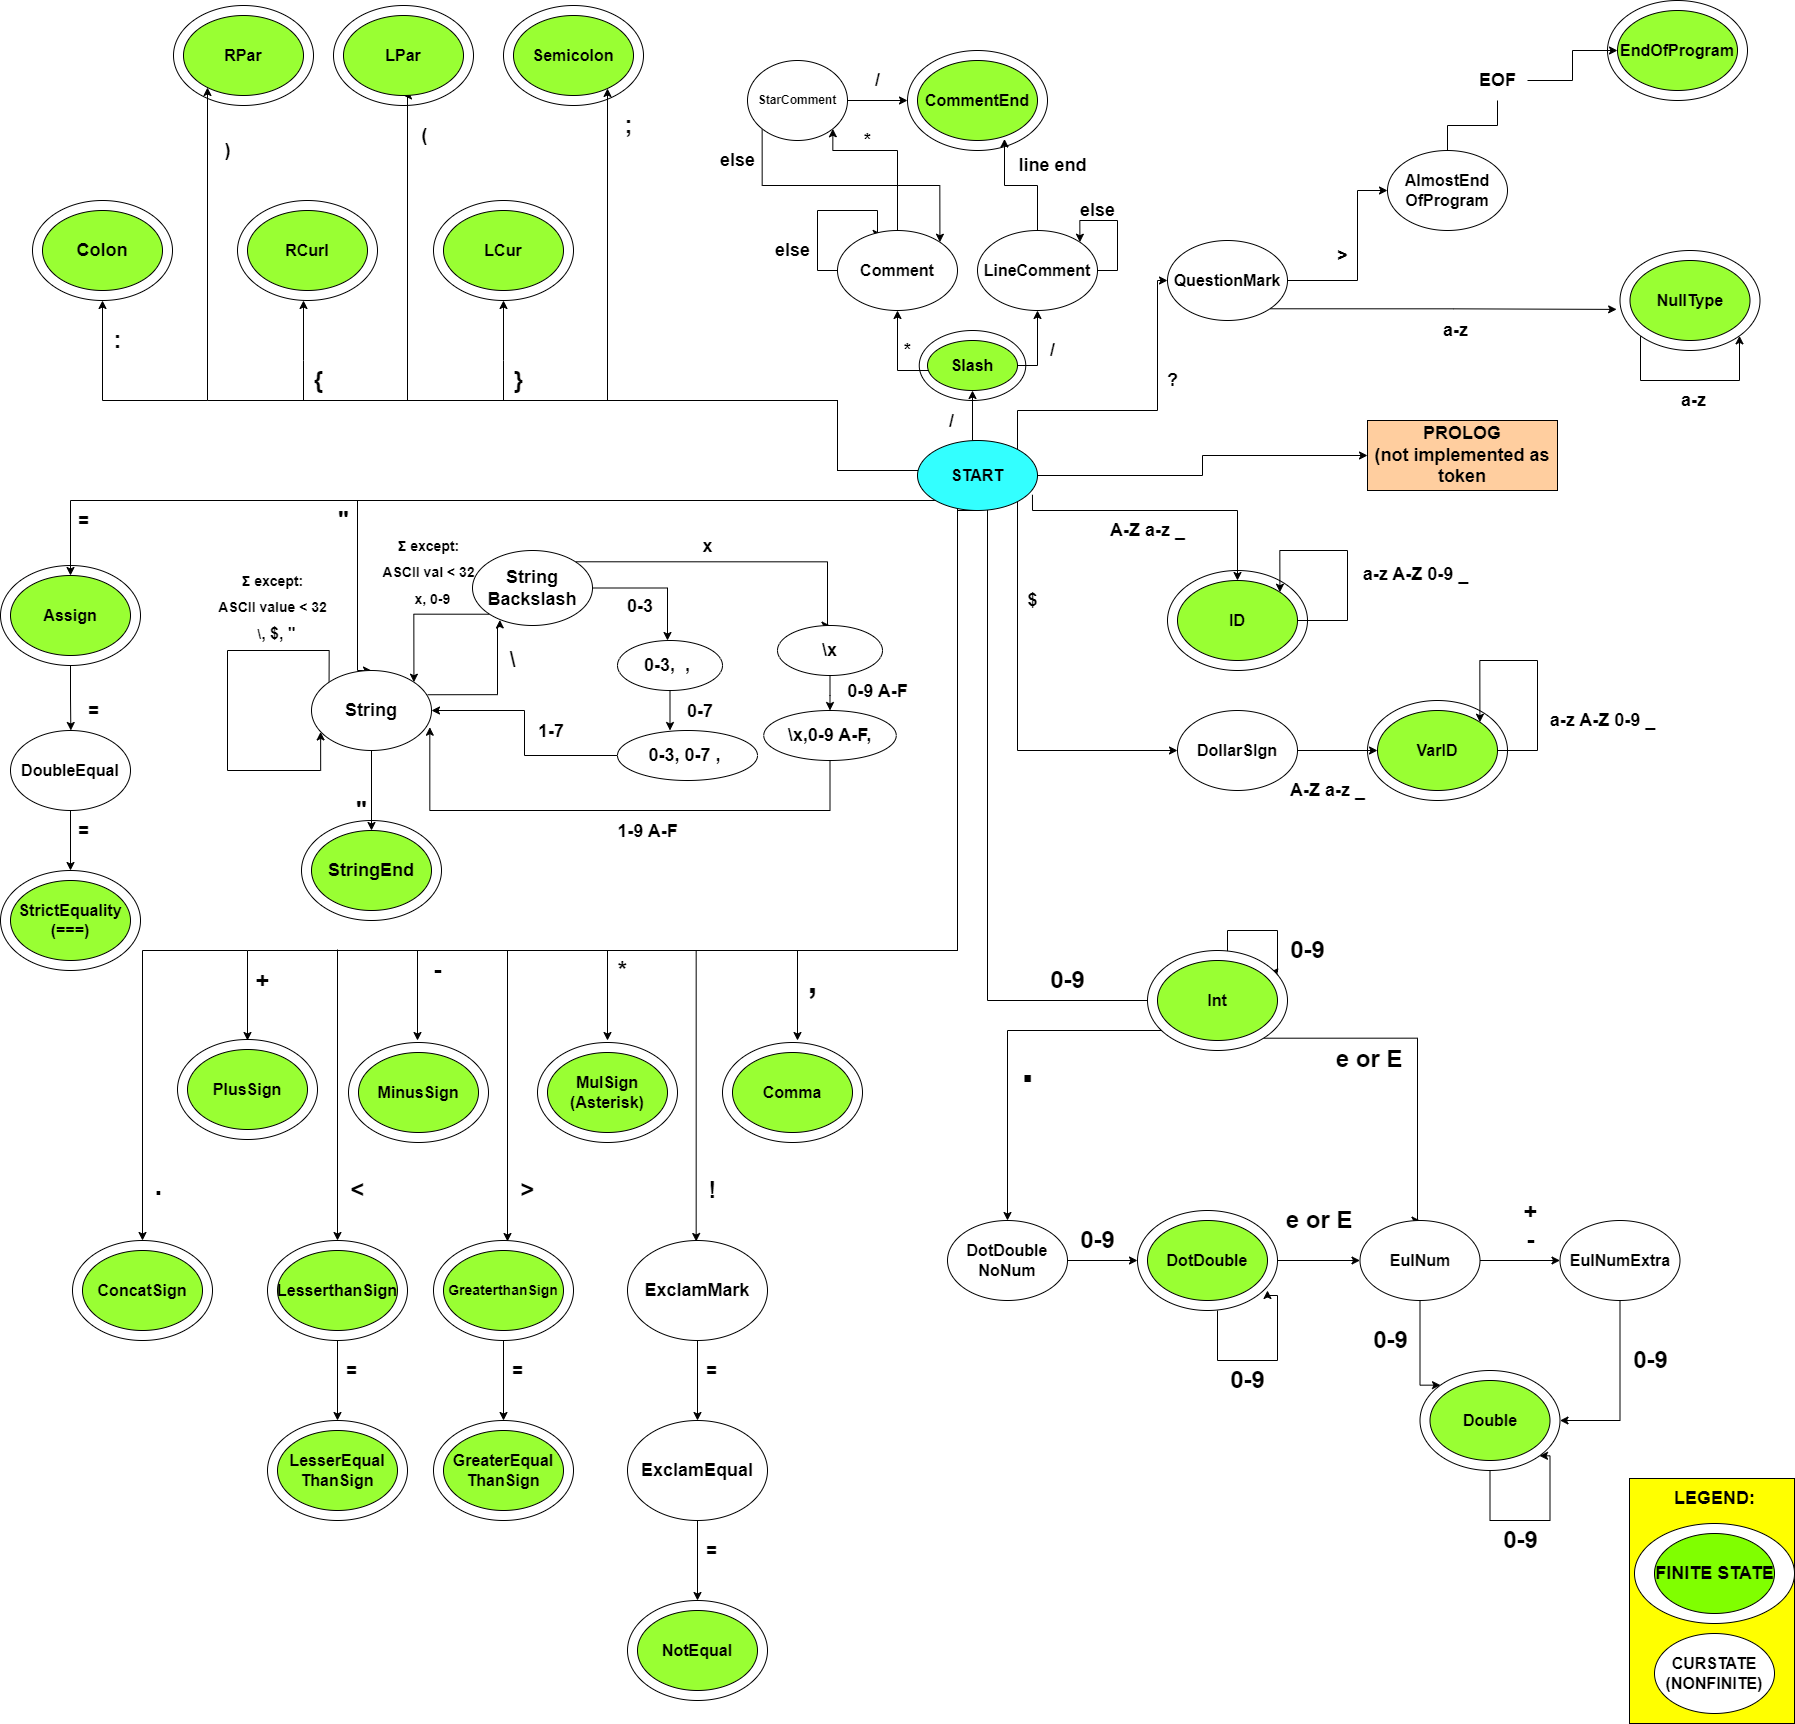
\includegraphics[width=\textwidth]{src/deterministicStateMachine_finall.png}
        \caption{Deterministický konečný automat stavů.}
        \label{Konecny automat}
    \end{figure}

    \begin{figure}[H]
        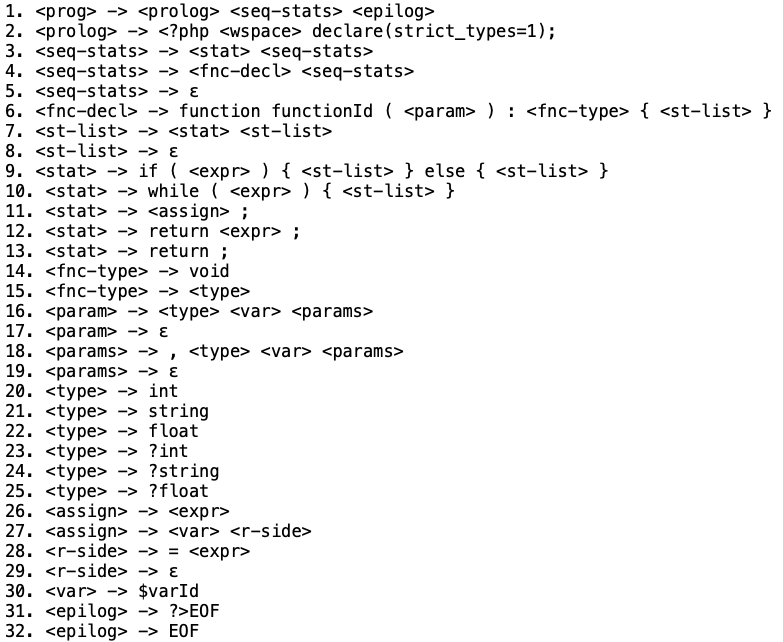
\includegraphics[width=0.65\textwidth]{src/LL-gramatika.png}
        \caption{LL gramatika.}
        \label{LL gramatika}
    \end{figure}

    \begin{figure}[H]
        \hspace*{-1cm}
        \centering
        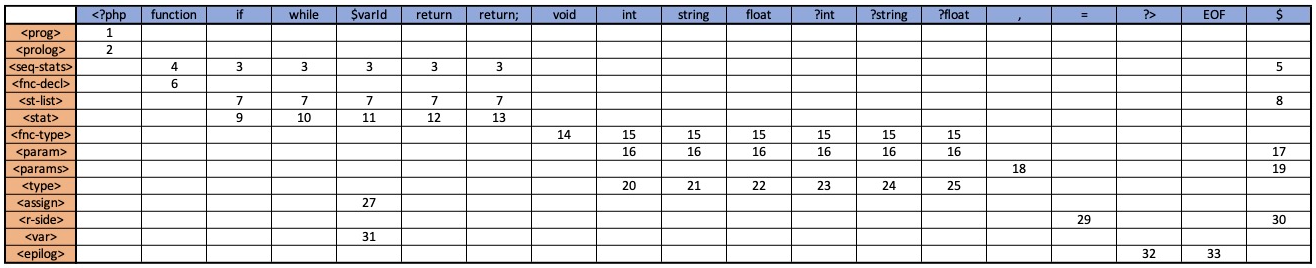
\includegraphics[width= 0.90 \paperwidth]{src/LL-tabulka.png}
        \caption{LL tabulka.}
        \label{LL tabulka}
    \end{figure}

    \begin{table}[H]
        \centering
        \begin{tabular}[p]{| l | c | c | c | c | c | c | c | c | c | c | c | c | c | c | c |}
            \hline
            &   \textbf{$\times$} & \textbf{$/$} & \textbf{$+$} & \textbf{$-$} & \textbf{$\cdot$} & \textbf{$<$} & \textbf{$>$} & \textbf{{$\geq$}} & \textbf{$\leq$} & \textbf{$\neq$} & \textbf{$=$} & \textbf{$($} & \textbf{$)$} & \textbf{$i$} & \textbf{\$} \\
            \hline
            \textbf{$\times$} &
                $>$ & $>$ & $>$ & $>$ & $>$ & $>$ & $>$ & $>$ & $>$ & $>$ & $>$ & $<$ & $>$ & $<$ & $>$ \\
            \textbf{$/$} &
                $>$ & $>$ & $>$ & $>$ & $>$ & $>$ & $>$ & $>$ & $>$ & $>$ & $>$ & $<$ & $>$ & $<$ & $>$ \\
            \textbf{$+$} &
                $<$ & $<$ & $>$ & $>$ & $>$ & $>$ & $>$ & $>$ & $>$ & $>$ & $>$ & $<$ & $>$ & $<$ & $>$ \\
            \textbf{$-$} &
                $<$ & $<$ & $>$ & $>$ & $>$ & $>$ & $>$ & $>$ & $>$ & $>$ & $>$ & $<$ & $>$ & $<$ & $>$ \\
            \textbf{$\cdot$} &
                $<$ & $<$ & $>$ & $>$ & $>$ & $>$ & $>$ & $>$ & $>$ & $>$ & $>$ & $<$ & $>$ & $<$ & $>$ \\
            \textbf{$<$} &
                $<$ & $<$ & $<$ & $<$ & $<$ &     &     &     &     & $>$ & $>$ & $<$ & $>$ & $<$ & $>$ \\
            \textbf{$>$} &
                $<$ & $<$ & $<$ & $<$ & $<$ &     &     &     &     & $>$ & $>$ & $<$ & $>$ & $<$ & $>$ \\
            \textbf{$\geq$} &
                $<$ & $<$ & $<$ & $<$ & $<$ &     &     &     &     & $>$ & $>$ & $<$ & $>$ & $<$ & $>$ \\
            \textbf{$\leq$} &
                $<$ & $<$ & $<$ & $<$ & $<$ &     &     &     &     & $>$ & $>$ & $<$ & $>$ & $<$ & $>$ \\
            \textbf{$\neq$} &
                $<$ & $<$ & $<$ & $<$ & $<$ & $<$ & $<$ & $<$ & $<$ &     &     & $<$ & $>$ & $<$ & $>$ \\
            \textbf{$=$} &
                $<$ & $<$ & $<$ & $<$ & $<$ & $<$ & $<$ & $<$ & $<$ &     &     & $<$ & $>$ & $<$ & $>$ \\
            \textbf{$($} &
                $<$ & $<$ & $<$ & $<$ & $<$ & $<$ & $<$ & $<$ & $<$ & $<$ & $<$ & $<$ & $=$ & $<$ &     \\
            \textbf{$)$} &
                $>$ & $>$ & $>$ & $>$ & $>$ & $>$ & $>$ & $>$ & $>$ & $>$ & $>$ &     & $>$ &     & $>$ \\
            \textbf{$i$} &
                $>$ & $>$ & $>$ & $>$ & $>$ & $>$ & $>$ & $>$ & $>$ & $>$ & $>$ &     & $>$ &     & $>$ \\
            \textbf{$\$$} &
                $<$ & $<$ & $<$ & $<$ & $<$ & $<$ & $<$ & $<$ & $<$ & $<$ & $<$ & $<$ &     & $<$ &     \\
            \hline
        \end{tabular}
        \caption{Precedenční tabulka.}
        \label{tabulka precedence}
    \end{table}
\end{document}
